
\subsection{Assessing System Reliability}
\label{reliability}







The supervision tree principle is adopted by Erlang and Akka users in the 
hope of improving the reliability of software applications.  Apart from the 
reported nine "9"s reliability of the Ericsson AXD 301 switch 
\citep{ArmstrongAXD} and the wide range of Akka use cases, how can software 
developers assure the reliability of their newly-implemented applications?  

TAkka is shipped with a Chaos Monkey library and a Supervision View library for 
assessing the reliability of TAkka applications.  A Chaos Monkey test randomly 
kills actors in a supervision tree and a Supervision View test dynamically 
captures the structure of supervision trees.  With the help of Chaos Monkey and 
Supervision View, users can visualize how their TAkka applications react to 
adverse conditions. 
% Missing nodes in the supervision tree (Section 
% \ref{calculator_chaos_test}) show that failures occur during the test. On the 
% other hand, any failed actors are restored, and hence appropriately 
% supervised applications (Section\ref{bencherl_chaos_test})  pass Chaos Monkey 
% tests.
We expected that appropriately supervised actors will be restored when they 
fails, and hence pass Chaos Monkey tests.

\begin{table*}
\begin{tabular}{| c | p{5 cm} | p{8.8 cm} | }
\hline
Mode & Failure & Description \\
\hline
Random (Default) & Random Failures & Randomly choose one of the other modes in 
each run. \\
\hline
Exception & Raise an exception & A victim actor randomly raises an exception 
from 
a user-defined set of exceptions. \\
\hline
Kill & Failures that can be recovered by scheduling service restart &  
Terminate 
a victim actor.  The victim actor can be restarted later. \\
\hline
PoisonKill & Unidentifiable failures & Permanently terminate a victim actor.  
The victim cannot be restarted.  \\ 
\hline 
NonTerminate & Design flaw or network congestion & Let a victim actor run 
into an infinite loop.  The victim actor consumes system resources but cannot 
process any messages. \\
\hline

\end{tabular}
\label{chaos}
\caption{TAkka Chaos Monkey Modes}
\end{table*}


\subsubsection {Chaos Monkey and Supervision View}

A Chaos Monkey test \citep{ChaosMonkey} randomly kills Amazon EC2 instances in 
an Auto Scaling Group.  In a Chaos Monkey test, the 
reliability of an application is tested against intensive adverse 
conditions.  Chaos Monkey is ported into Erlang to detect potential flaws of 
supervision trees \citep{ErlangChaosMonkey}.  We port the Erlang version of 
Chaos 
Monkey into the TAkka library.  In addition to randomly killing actors, users 
can simulate other common failures by using other modes in Table \ref{chaos}.


To dynamically monitor changes of supervision trees, we design and implement 
a Supervision View library. In a supervision view test, an instance of {\tt 
ViewMaster} periodically sends request messages to interested actors.  At the 
time when the request message is received, an active TAkka actor replies wih 
its status to the {\tt ViewMaster} instance and passes the request message to 
its children.  The status message includes its actor path, the paths of its 
children, and the time when the reply is sent.  The {\tt ViewMaster} instance 
records status messages and passes them to a visualizer, which will analyze 
and 
interpret changes of the tree structure during the testing period.  We believe 
that a similar library can be straightforwardly implemented in actor systems such 
as Akka and Erlang.  From a practical point of view, the dynamic actor 
monitoring overcomes the two limitations of the static analyses tool 
developed in Nyström's PhD thesis \citep{JanHenry}, which only applies to 
applications built using the Erlang/OTP library and cannot tell whether 
an actor will actually be started at runtime.



\begin{comment}
 
% save pages
\subsubsection{A Partly Failed Safe Calculator}
\label{calculator_chaos_test}

In the hope that Chaos Monkey and Supervision View tests can reveal breaking 
points of a supervision tree, we modify the Safe Calculator example and run a 
test as follows.  Firstly, we run three safe calculators on three Beowulf 
nodes, under the supervision of a root actor using the {\tt OneForOne} strategy 
with {\tt Restart} action.  Secondly, we set different supervisor strategies 
for each safe calculator.  The first safe calculator, S1, restarts any failed 
child immediately.  This configuration simulates a quick restart process.
The second safe calculator, S2, computes a Fibonacci number in a naive way for 
about 10 seconds before restarting any failed child.  This configuration 
simulates 
a restart process which may take a noticeable time.  The third safe calculator, 
S3, stops the child when it fails.  Finally, we set-up the a Supervision View 
test which captures the supervision tree every 15 seconds, and a Chaos Monkey 
test which tries to kill a random child calculator every 3 seconds.

A test result, given in Figure \ref{fig:supervisionview}, gives the expected
tree structure at the beginning, 15 seconds and 30 seconds of the test.  Figure 
\ref{fig:tree1} shows that the application initialized three safe calculators as 
described.  In Figure \ref{fig:tree2}, S2 and its child are marked as dashed 
circles because it takes the view master more than 5 seconds to receive their 
responses.  From the test result itself, we cannot tell whether the delay is 
due to a blocked calculation or a network congestion.  Comparing to Figure 
\ref{fig:tree1}, the child of S3 is not shown in Figure \ref{fig:tree2} and 
Figure \ref{fig:tree3} because no response is received from it until the end of 
the test.  When the test ends, no response to the last request is received 
from S2 and its child.  Therefore, both S2 and its child are not shown in 
Figure \ref{fig:tree3}.  S1 and its child appear in all three Figures because 
either they never fail during the test or they are recovered from failures 
within a short time.

\begin{figure}[h]
     \begin{center}
        \subfigure[]{
            \label{fig:tree1}
            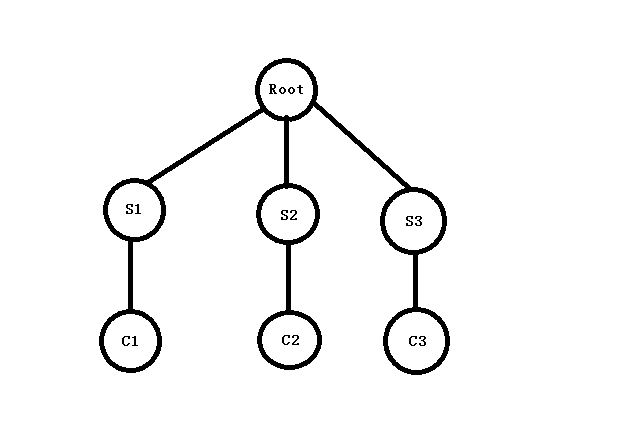
\includegraphics[scale=0.23]{Tree1.png}
        }
        \subfigure[]{
           \label{fig:tree2}
           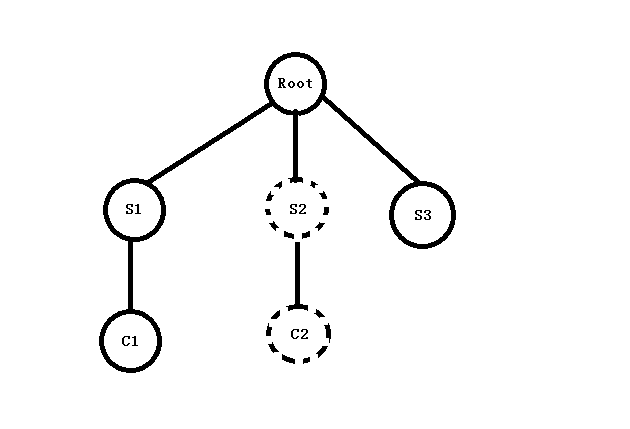
\includegraphics[scale=0.23]{Tree2.png}
        }
        \subfigure[]{
            \label{fig:tree3}
            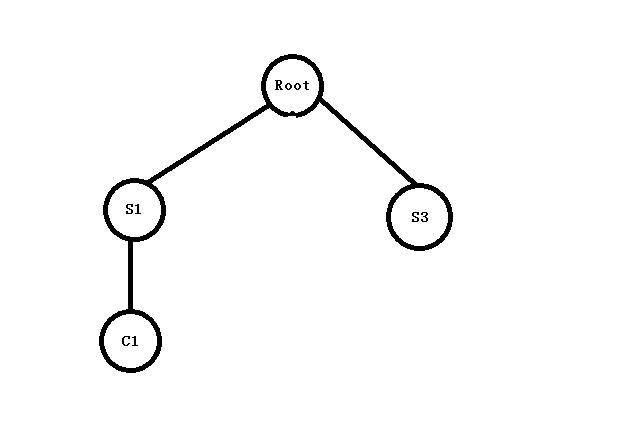
\includegraphics[scale=0.23]{Tree3.png}
        }
    \end{center}
    \caption{Supervision View Example}
   \label{fig:supervisionview}
\end{figure}


\end{comment}

\subsubsection{BenchErl Examples with Different Supervisor Strategies}
\label{bencherl_chaos_test}

To test the behaviour of applications with internal states under 
different supervisor strategies, we apply the {\tt OneForOne} supervisor 
strategy with different failure actions to the 6 BenchErl examples and test 
those examples using Chaos Monkey and Supervision View.  The master node of 
each BenchErl test is initialized with an internal counter.  The internal 
counter decrease when the master node receives a finishing messages from its 
children.  The test application stops when the internal counter of the master 
node reaches 0.  We set the Chaos Monkey test with the {\tt Kill} mode and 
randomly kill a victim actor every second.  When the {\tt Escalate} action is 
applied to the master node, the test stops as soon as the first {\tt Kill} 
message sent from the Chaos Monkey test.  When the {\tt Stop} action is applied, 
the application does not stop and, eventually, the supervision view test only 
receives messages from the master node.  When the {\tt Restart} action is 
applied, the application does not stop but the Supervision View test receives 
messages from the master node and its children.  When the {\tt Resume} action is 
applied, all tests stop eventually with a longer run-time comparing to tests 
without Chaos Monkey and Supervision View tests.


